\documentclass[a4paper, british]{article}

\usepackage[utf8]{inputenc}
\usepackage[T1]{fontenc}
\usepackage{babel}
% \usepackage[margin=2.5cm,a4paper]{geometry}
% \usepackage[skip=1em]{parskip}
\usepackage{lmodern} 
\usepackage{microtype}
% \usepackage{xcolor}
\usepackage{graphicx}
\graphicspath{ {./figures/} }
\usepackage{float}
% \usepackage{enumitem}
\usepackage{adjustbox} % rescale - useful for Dia exported TeX
\usepackage{tikz}
% \usepackage{pgfplots}
\usepackage{booktabs} %tables no vertical lines
% \usepackage{array}
% \usepackage{authblk}
% \usepackage{fancyhdr} %headers and footers
% \usepackage{titlesec}
% \usepackage{tcolorbox} % framed text boxes
% \usepackage{mathtools, amssymb, amsthm}
% \usepackage{gensymb}
\usepackage{chemformula} % chemical formulae
\usepackage{chemfig} % molecular figures
\usepackage{siunitx}
\usepackage{csquotes}
\usepackage[titletoc, title]{appendix}
% \usepackage{lettrine} % initials

\usepackage[
pdfauthor={Adam Menne},
pdftitle={Chemistry 254 - Practical 5},
pdfsubject={},
pdfkeywords={}]{hyperref}

\usepackage[noabbrev]{cleveref}

\usepackage[
backend=biber,
style=numeric,
sorting=none,
doi=true,
isbn=false
]{biblatex}
\addbibresource{citations.bib}

\setlength{\parskip}{1em}
\setlength{\parindent}{0em}
\linespread{1.3}

\title{Chemistry 254\\ Experiment 5\\ Adsorption}
\date{Last edited on \today}
\author{Adam Menne\\ Stellenbosch University}

\begin{document}

\maketitle

\begin{abstract}
\noindent
In this practical the adsorption of acetic acid on activated carbon was measured at various concentrations. These empirical values were then used to determine the suitability of different adsorption isotherms
\end{abstract}

\tableofcontents

\newpage


\section{Results}

The initial and equilibrium concentrations for acetic acid are shown in \cref*{tab:conc}. The mass of acetic acid adsorbed onto the charcoal in \cref*{tab:mass}.

\Cref*{fig:f1} and \cref*{fig:f2} show the linear regressions giving parameters to the Freundlich and Langmuir isotherms.

\begin{table}[H]
    \centering
    \caption{Acetic acid concentrations}
    \vspace*{2mm}
    \label{tab:conc}
    \begin{tabular}{cll}
    \toprule
    Sample & Initial (M) & Equilibrium (M) \\ \midrule
    1 & 0.4052 & 6.93079e-5 \\
    2 & 0.3578 & 6.14219e-5 \\
    3 & 0.1483 & 2.65236e-5 \\
    4 & 0.1065 & 4.61498e-5 \\
    5 & 0.07732 & 3.40209e-5 \\
    6 & 0.05023 & 4.36507e-5 \\
    7 & 0.02005 & 1.85265e-5 \\ \bottomrule
\end{tabular}
\end{table}

\begin{table}[H]
    \centering
    \caption{Mass of acetic acid adsorbed on charcoal}
    \vspace*{2mm}
    \label{tab:mass}
    \begin{tabular}{cl}
    \toprule
    Sample & Mass adsorbed (m) \\ \midrule
    1 & 0.0007543 \\
    2 & 0.0003504 \\
    3 & 0.00027 \\
    4 & 0.0001598 \\
    5 & 0.0001142 \\
    6 & 3.871e-5 \\
    7 & 2.265e-5
    \end{tabular}
    \end{table}



\begin{figure}[H]
    \centering
    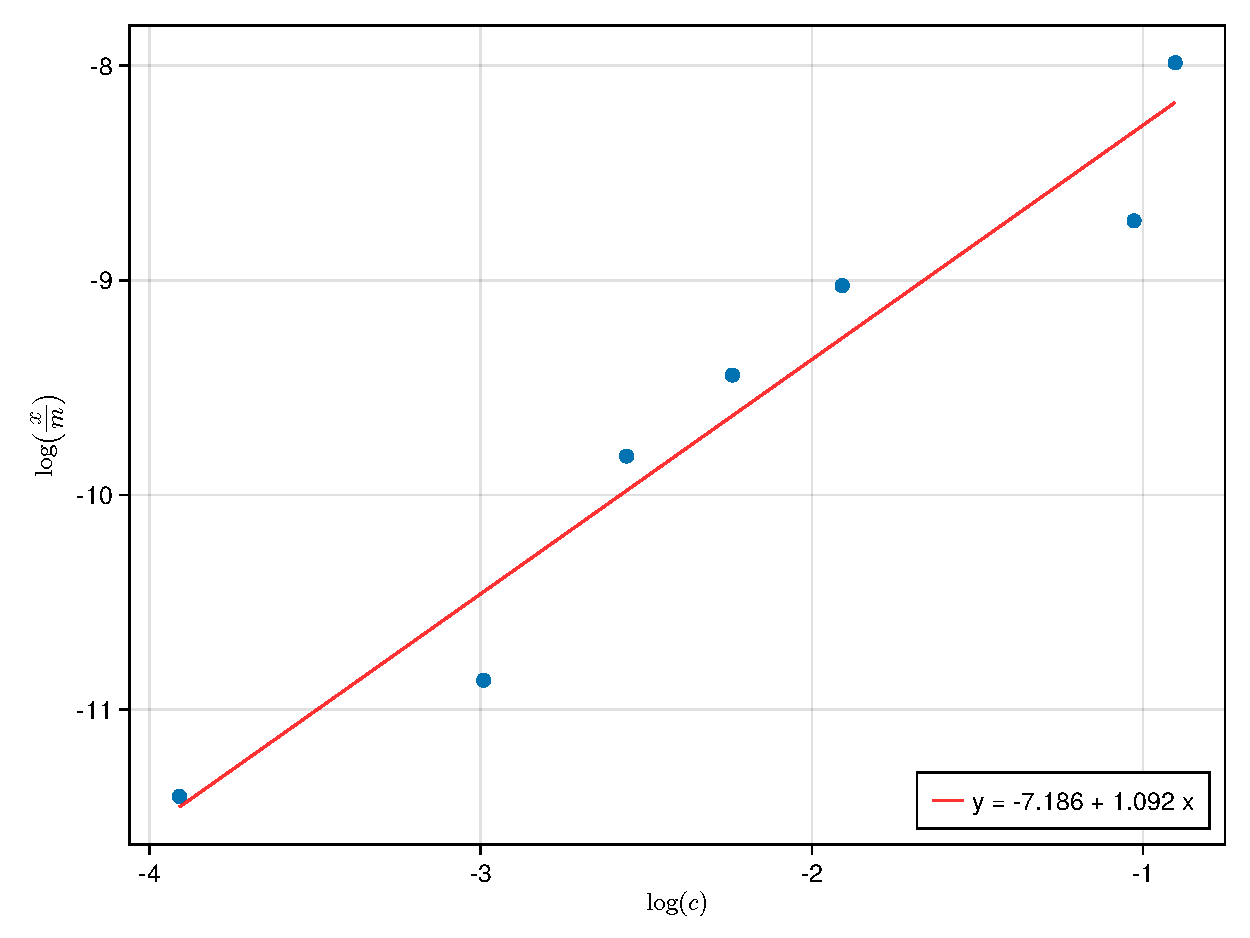
\includegraphics[width=\textwidth]{figures/f1.pdf}
    \caption{Freundlich isotherm}
    \label{fig:f1}
\end{figure}

\begin{figure}[H]
    \centering
    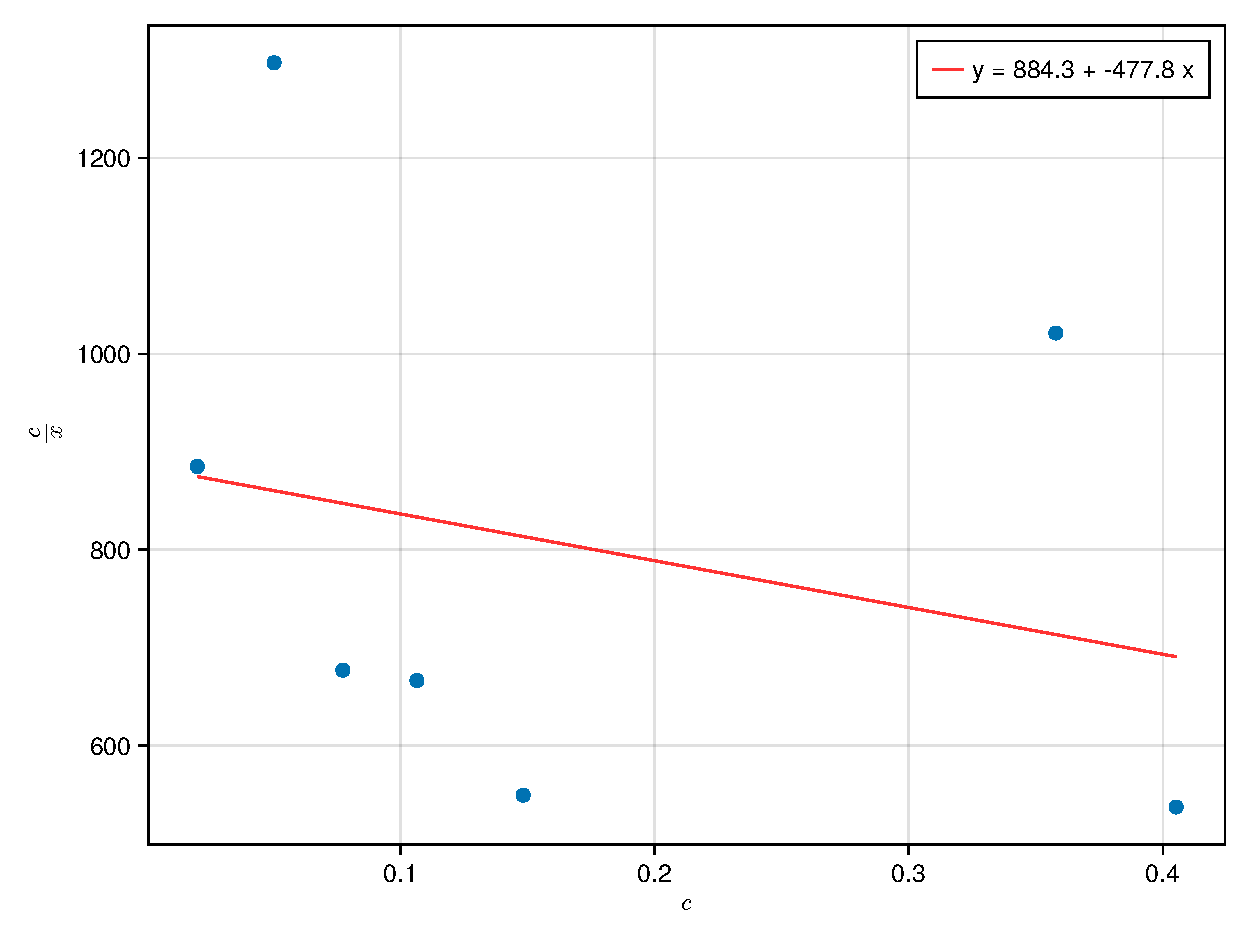
\includegraphics[width=\textwidth]{figures/f2.pdf}
    \caption{Langmuir isotherm}
    \label{fig:f2}
\end{figure}



A static export of the notebook containing all analysis and figures is available at \url{https://adammenne.github.io/chemistry_254/practical_5/notebook.html}.\\ With full source code available at \url{https://github.com/AdamMenne/chemistry_254/tree/master/practical_5}

\section{Discussion}

The Freundlich isotherm had a significantly better correlation coefficient with a value 0.942 of compared to 0.0684 the achieved by the Langmuir isotherm. This shows the inability of the Langmuir isotherm to account for materials in which multiple layers of adsorption can occur. 

Accuracy could be increased with a larger and wider sample size, as there were notable discrepancies for samples that were titrated multiple times.

\newpage

\begin{appendices}

\section{Additional tasks}

\begin{enumerate}
    \item The Freundlich isotherm
    \item That it is a physical adsorption and multiple layers are adsorbed 
    \item \(\frac{1}{x_m} = -4.778\) and \(\frac{1}{Kx_m} = 185.08\)
    \item It allows us to account for error due to the titrant reacting with the solvent
    \item Exposure to suitably high temperatures such that all adsorbed materials will undergo volatilisation.
\end{enumerate}

\newpage

% \section{Flow Diagram}

% \begin{enumerate}
%     \item Heat a  25 \(cm^3\) pipette with a hair dryer, attach cotton filter, and fill past the mark
%     \item Remover filter, wipe off crystals, and evacuate the pipette to the mark
%     \item Empty into Erlenmeyer flask, washing with ethanol, add 2 to 3 drops phenolphthalein 
%     \item Titrate with 0.1 \(M\ NaOH\)
%     \item Clean pipette with ethanol followed by acetone, and dry
%     \item Repeat 3 times for both temperatures
% \end{enumerate}

\newpage

\section{MSDS}

\subsection*{Acetic acid}

\begin{itemize}
    \item Flammable, corrosive
    \item[-] causes skin burns and eye damage
    \item[-] if in contact with skin or eyes wash for several minutes  
\end{itemize}

\subsection*{Sodium hydroxide}

\begin{itemize}
    \item Corrosive
    \item[-] may cause skin burns, eye damage
    \item[-] if in contact with skin or eyes wash for several minutes  
\end{itemize}

\end{appendices}

\end{document}